\documentclass{beamer} 
\usetheme{Madrid}
\usepackage{pdfpages}
\usepackage[utf8x]{inputenc}
\usepackage{url}
\usepackage{graphicx}
\usepackage{graphics}
\usepackage{adjustbox}
\usepackage{ragged2e}
\usepackage{verbatim}
\usepackage{textpos}
\usepackage{lmodern,textcomp}
 \setbeamertemplate{enumerate items}[default]
 \setbeamertemplate{itemize items}[circle]
 \setbeamertemplate{frametitle continuation}{}
\setbeamertemplate{section in toc}[circle]
\setbeamertemplate{subsection in toc}[circle]

\usepackage{hyperref}
\hypersetup{
    colorlinks=true,
    linkcolor=,
    filecolor=magenta,      
    urlcolor=cyan,
}

\beamertemplatenavigationsymbolsempty
%%%%%%%%%%%%%%%Color%%%%%%%%%%%%%%%
\definecolor{KIPlum}{HTML}{880052}
\definecolor{box}{RGB}{250, 117, 144}
\usecolortheme[named=KIPlum]{structure}

%%%%%%%%%%%%%%%Bibliography setting%%%%%%%%%%%%%%%
\usepackage[numbers,comma,sort&compress]{natbib}
\makeatletter
\renewcommand{\@biblabel}[1]{#1.} %remove brackets from the ref list
\setcitestyle{comma, numbers,sort&compress, super}
\bibliographystyle{/Users/Enoch/survbib/bibtex/bst/vancouv12}
\setbeamertemplate{bibliography item}{text}

%%%%%%%%%%%%%%%Title page%%%%%%%%%%%%%%%

\title[Applied Epi I: Data Management]{Applied Epidemiology I: Data Management}
\date{\today}
\author[Enoch Yi-Tung Chen]{Enoch Yi-Tung Chen}
\institute[MEB]{Department of Medical Epidemiology and Biostatistics, Karolinska Insitutet}

%%%%%%%%%%%%%%\begin{document}%%%%%%%%%%%%%%%%

\begin{document}

\begin{frame}
\maketitle 
\end{frame}

%%%%%%%%%%%%%%Outline%%%%%%%%%%%%%%%%
\begin{frame}{Acknowledgements}
This course material in data management is based on my learning from \href{https://staff.ki.se/people/annajo}{Anna Johansson}'s \href{https://play.ki.se/media/Data+Management+and+research+documentation+for+researchers/0_h64ki6v7?_ga=2.131118287.1557257458.1589785892-1364153581.1557067020}{workshop at KI library}\footnote{This workshop is currently available on KI Play as well. }, teachings in \href{https://kiwas.ki.se/katalog/katalog/kurs/851;jsessionid=e42ee2c1f6b081f28bf83e3d0321?lang=en}{Good Data Management Practice in Epidemiological Research}, and MEB Guidelines for Documentation and Archiving Version 6 \footnote{The Department of Medical Epidemiology and Biostatistics, Karolinska Institutet. MEB Guidelines for Documentation and Archiving Version 6. 2018.}. I personally want to thank for their effort on education in data management.

\end{frame}

%%%%%%%%%%%%%%Outline%%%%%%%%%%%%%%%%
\begin{frame}
\addtolength{\leftskip}{1cm}
\begin{minipage}{\textwidth}
\vspace{0.5cm}
\frametitle{Outline}
    \tableofcontents[hideallsubsections]
\end{minipage}
\end{frame}

%%%%
\section{What if no data management?}
\begin{frame}[allowframebreaks]{What if no data management?}
In the beginning, 
\begin{center}
		
\includegraphics{image/desktop}
\end{center}

\newpage
In the half-way of the research, \\
\begin{center}
		
\includegraphics{image/messy-desktop}
\end{center}

\newpage
At the end, or saying you cannot even walk till the end?

\begin{center}
		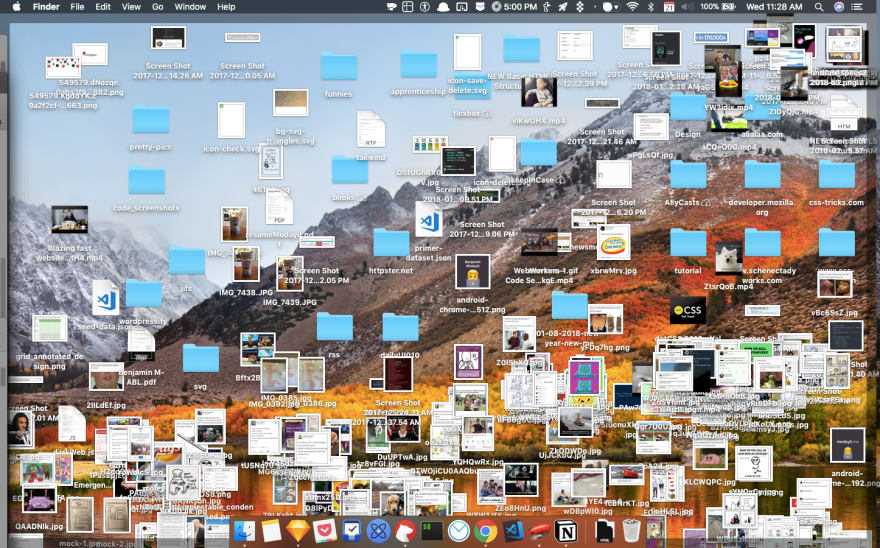
\includegraphics[scale=0.3]{image/more-messy-desktop}
\end{center}

\newpage

Imagine now...
\begin{itemize}
	\item if you want to correct Table I, where is the do file for descriptive analysis?
	\item if your supervisor says, "Please summarise how far you've gone in this project." You probably cannot just drop him/her your syntax. 
	\item if your classmate asks you to teach her how to write a certain Stata code, you remember you've done it before, but where did you put it?
	\item if your collaborator needs to take over your analysis, can he/she understand what you've completed?
\end{itemize}

\newpage 

\begin{center}
		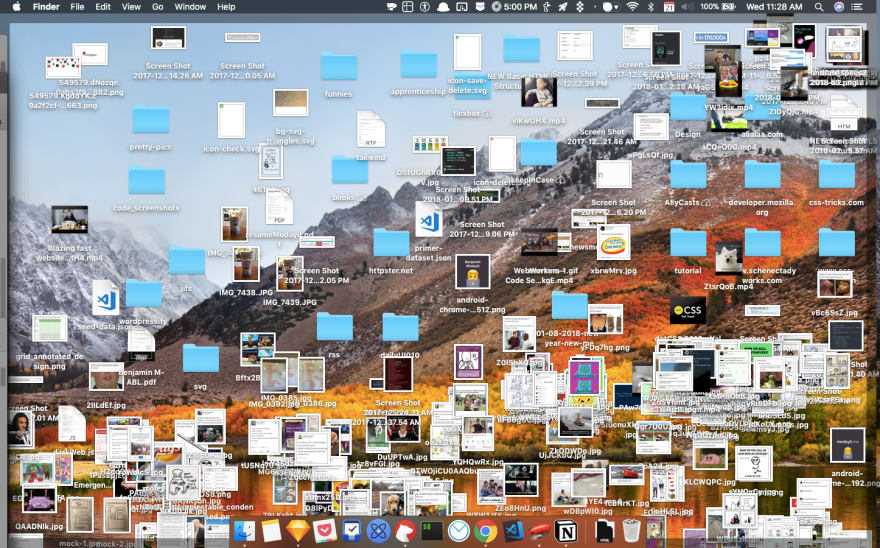
\includegraphics[scale=0.3]{image/more-messy-desktop}
\end{center}

\newpage

So I would say you need to have a friend called \\
\begin{center}
	{\huge \textbf{Data Management}}
\end{center}

\end{frame}

%%%%
\section{Aims of data management}
\begin{frame}{Aims of data management}
\begin{itemize}
	\item To ensure the analysis is reproducible
	\item To work coherently and efficiently with yourself 
	\item To ensure the project can be understood by others (supervisors, collaborators, and future readers)
	\item To create a good work flow and enhance accuracy of work 	
\end{itemize}
\end{frame}

%%%%
\section{Good folder structure}
\begin{frame}{Good folder structure}
	\begin{columns}
	\begin{column}{0.5\textwidth}
	The core elements of folders are listed below:
		\begin{itemize}
				\item Data
				\item Documents
				\item Log
				\item Output
				\item Program
		\end{itemize}
	\end{column}
	
	\begin{column}{0.5\textwidth}
	\begin{figure}
			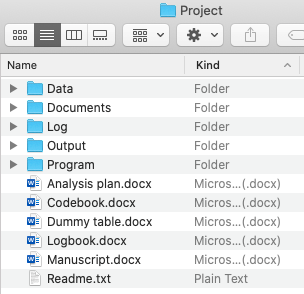
\includegraphics[scale=0.4]{image/structure}
			\caption{Good project folder structure. (Please bear with me that I am Mac user!)}
	\end{figure}
	\end{column}
	\end{columns}

\end{frame}

%%%%
\section{Good documents}
	\begin{frame}{Good documents}
	\begin{columns}
	\begin{column}{0.5\textwidth}
	Besides good folder structure, you should also consider keeping good documents
		\begin{itemize}
				\item Analysis plan
				\item Codebook\footnotemark
				\item Dummy table
				\item Logbook\footnotemark[\value{footnote}]
				\item Manuscript
		\end{itemize}
	
	\end{column}
	
	\begin{column}{0.5\textwidth}
	\begin{figure}
			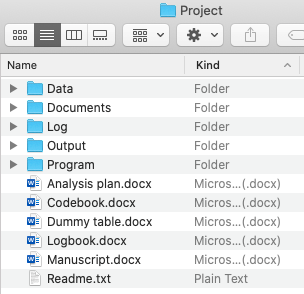
\includegraphics[scale=0.4]{image/structure}
			\caption{Good project folder structure.}
	\end{figure}
	\end{column}
	\end{columns}
	\footnotetext[3]{can be included in analysis plan as well}
\end{frame}

%%%%
\section{Good Readme.txt}	
\begin{frame}{Good Readme.txt}
\begin{columns}
	\begin{column}{0.5\textwidth} 
	\begin{itemize}
	\item You should illustrate how to use these documents/folders in the Readme.txt. 
	\item  A good Readme.txt is a good tourist guide in this project folder.

	\end{itemize}
	\end{column}
	
	\begin{column}{0.5\textwidth}
	\begin{figure}
			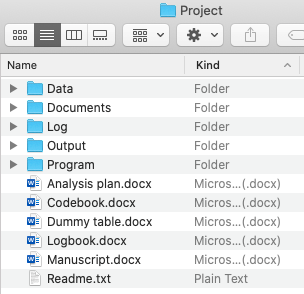
\includegraphics[scale=0.4]{image/structure}
			\caption{Good project folder structure.}
	\end{figure}
	\end{column}
	\end{columns}
\end{frame}

%%%%
\section{Good habits on coding}
\begin{frame}[allowframebreaks]{Good habit on coding}
\begin{columns}
	\begin{column}{0.3\textwidth} 
	\begin{itemize}
	\item log on
	\item[] 
	\item Filename
	\item Study
	\item Created
	\item Updated
	\item Purpose
	\item Note
	\item[] 
	\item \textbf{Start your code}
	\item[] 
	\item log close
	\end{itemize}
	\end{column}
	
	\begin{column}{0.7\textwidth} 
			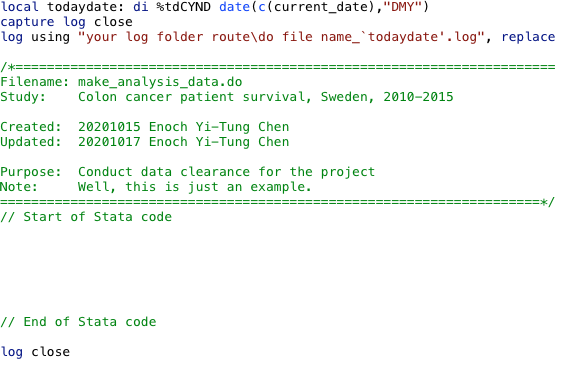
\includegraphics[scale=0.5]{image/header}
	\end{column}

\end{columns}

\newpage

\begin{itemize}
	\item Talk to yourself what you are doing.
	\item You've got a friend in me! (Parallel analysis)
	\item Rubber duck debugging
	\item[] 
	\item[] \centering 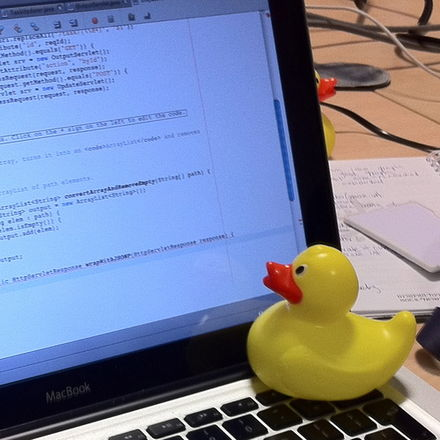
\includegraphics[scale=0.3]{image/rubberduck}
\end{itemize}

\end{frame}

%%%%
\section{Other do's and don'ts}

\begin{frame}{Other do's and don'ts}
	\begin{enumerate}
	\item Use a shared drive. (Sometimes you are even required to do that because of data privacy.)
	\item Give appropriate names to your files and variables	
	\begin{itemize}
		\item No stupid names, such as new1, new2, new3, final1, final2, final3, latest1
		\item No space in-between & No special character (in case, the software cannot read.)
		\item For binomial variables, $=1$ implies yes, and $=0$ implies no.
		\item Label your variables, please!
	\end{itemize}
	\item Same names for linking files (.do .r .sas $\rightarrow$ .log $\rightarrow$ .doc)
	\item Don't replace the original files or variables. (Well if you accidentally do this, you still get a chance to revert if using shared drive.)
	\end{enumerate}

\end{frame}

\section{Wrap it up}
\begin{frame}{Wrap it up}
\begin{itemize}
\item In summary, a good data management contains GOOD
\begin{enumerate}
	\item folder structure
	\item documents
	\item readme
	\item habits
\end{enumerate}

\item How can this lecture help you? \\
\item I attached the resources you can use for DM your current and future projects.
\end{itemize}
\end{frame}

\section{References}
\begin{frame}{References}
\begin{itemize}
	\item	
\end{itemize}
\end{frame}
\end{document}